\begin{figure}[t!]
\centering
\vspace{-5px}
%
\includegraphics[scale=.5]{img/optimization_intro_revised.pdf}
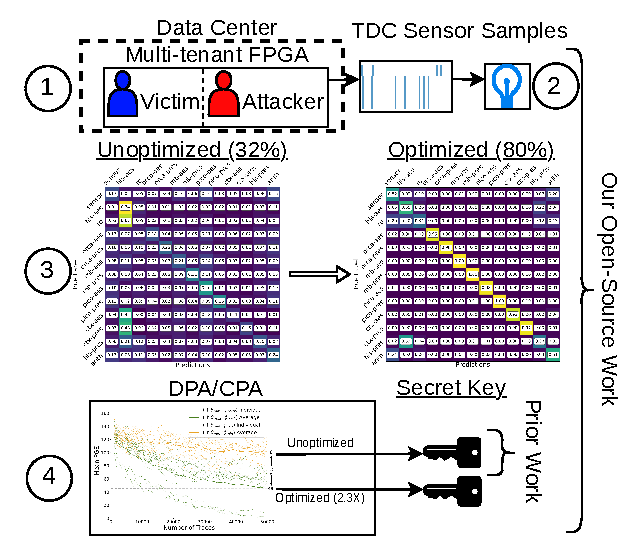
\includegraphics[scale=.85]{img/ASPLOS_Big_Picture.pdf}
\vspace{-10px}
\caption{\textcircled{\raisebox{-.8pt} {1}} An attacker spatiotemporally locates with a victim. % to extract information about the victim's computation. 
\textcircled{\raisebox{-.8pt} {2}} The attacker instantiates our \name TDC. % that measures the shared power distribution network. 
\textcircled{\raisebox{-.8pt} {3}} Our dynamic tuning techniques improve the ability to classify victim co-tenant computation by 2.5$\times$. \textcircled{\raisebox{-.8pt} {4}} After recognizing a cryptographic core, dynamic tuning increases the effectiveness of correlation power analysis by 2.2$\times$.
%\dr{Where did spatiotemporally come from? It would be cool to sneak 2.5x and 2.2x into the figure.} \cd{I do not know who added spatiotemporally, but it makes sense to me. Figure updated.} \rk{Guilty! I also learned that spatiotemporal and temporospatial are both words that seem to be equivalent? Happy to be educated on the difference. We should probably settle on one or the other if we are using both.}
%Stages 1-4 provide a pipeline for optimizing side channel sensor readings, correctly determining co-located computation, and performing a key recovery attack. }
%\cd{TODO - squish if possible. Open source hyphenated?
}
\label{fig:intro_fig}
\vspace{-10px}
\end{figure}